Das ALICE Experiment wurde speziell zur Untersuchung des Quark-Gluonen-Plasmas gebaut.
Um die Anspr\"uche daf\"ur besonders gut erf\"ullen zu k\"onnen besteht das ALICE Experiment aus einer Vielzahl unterschiedlicher Detektoren.
\begin{figure}[thp]
\centering
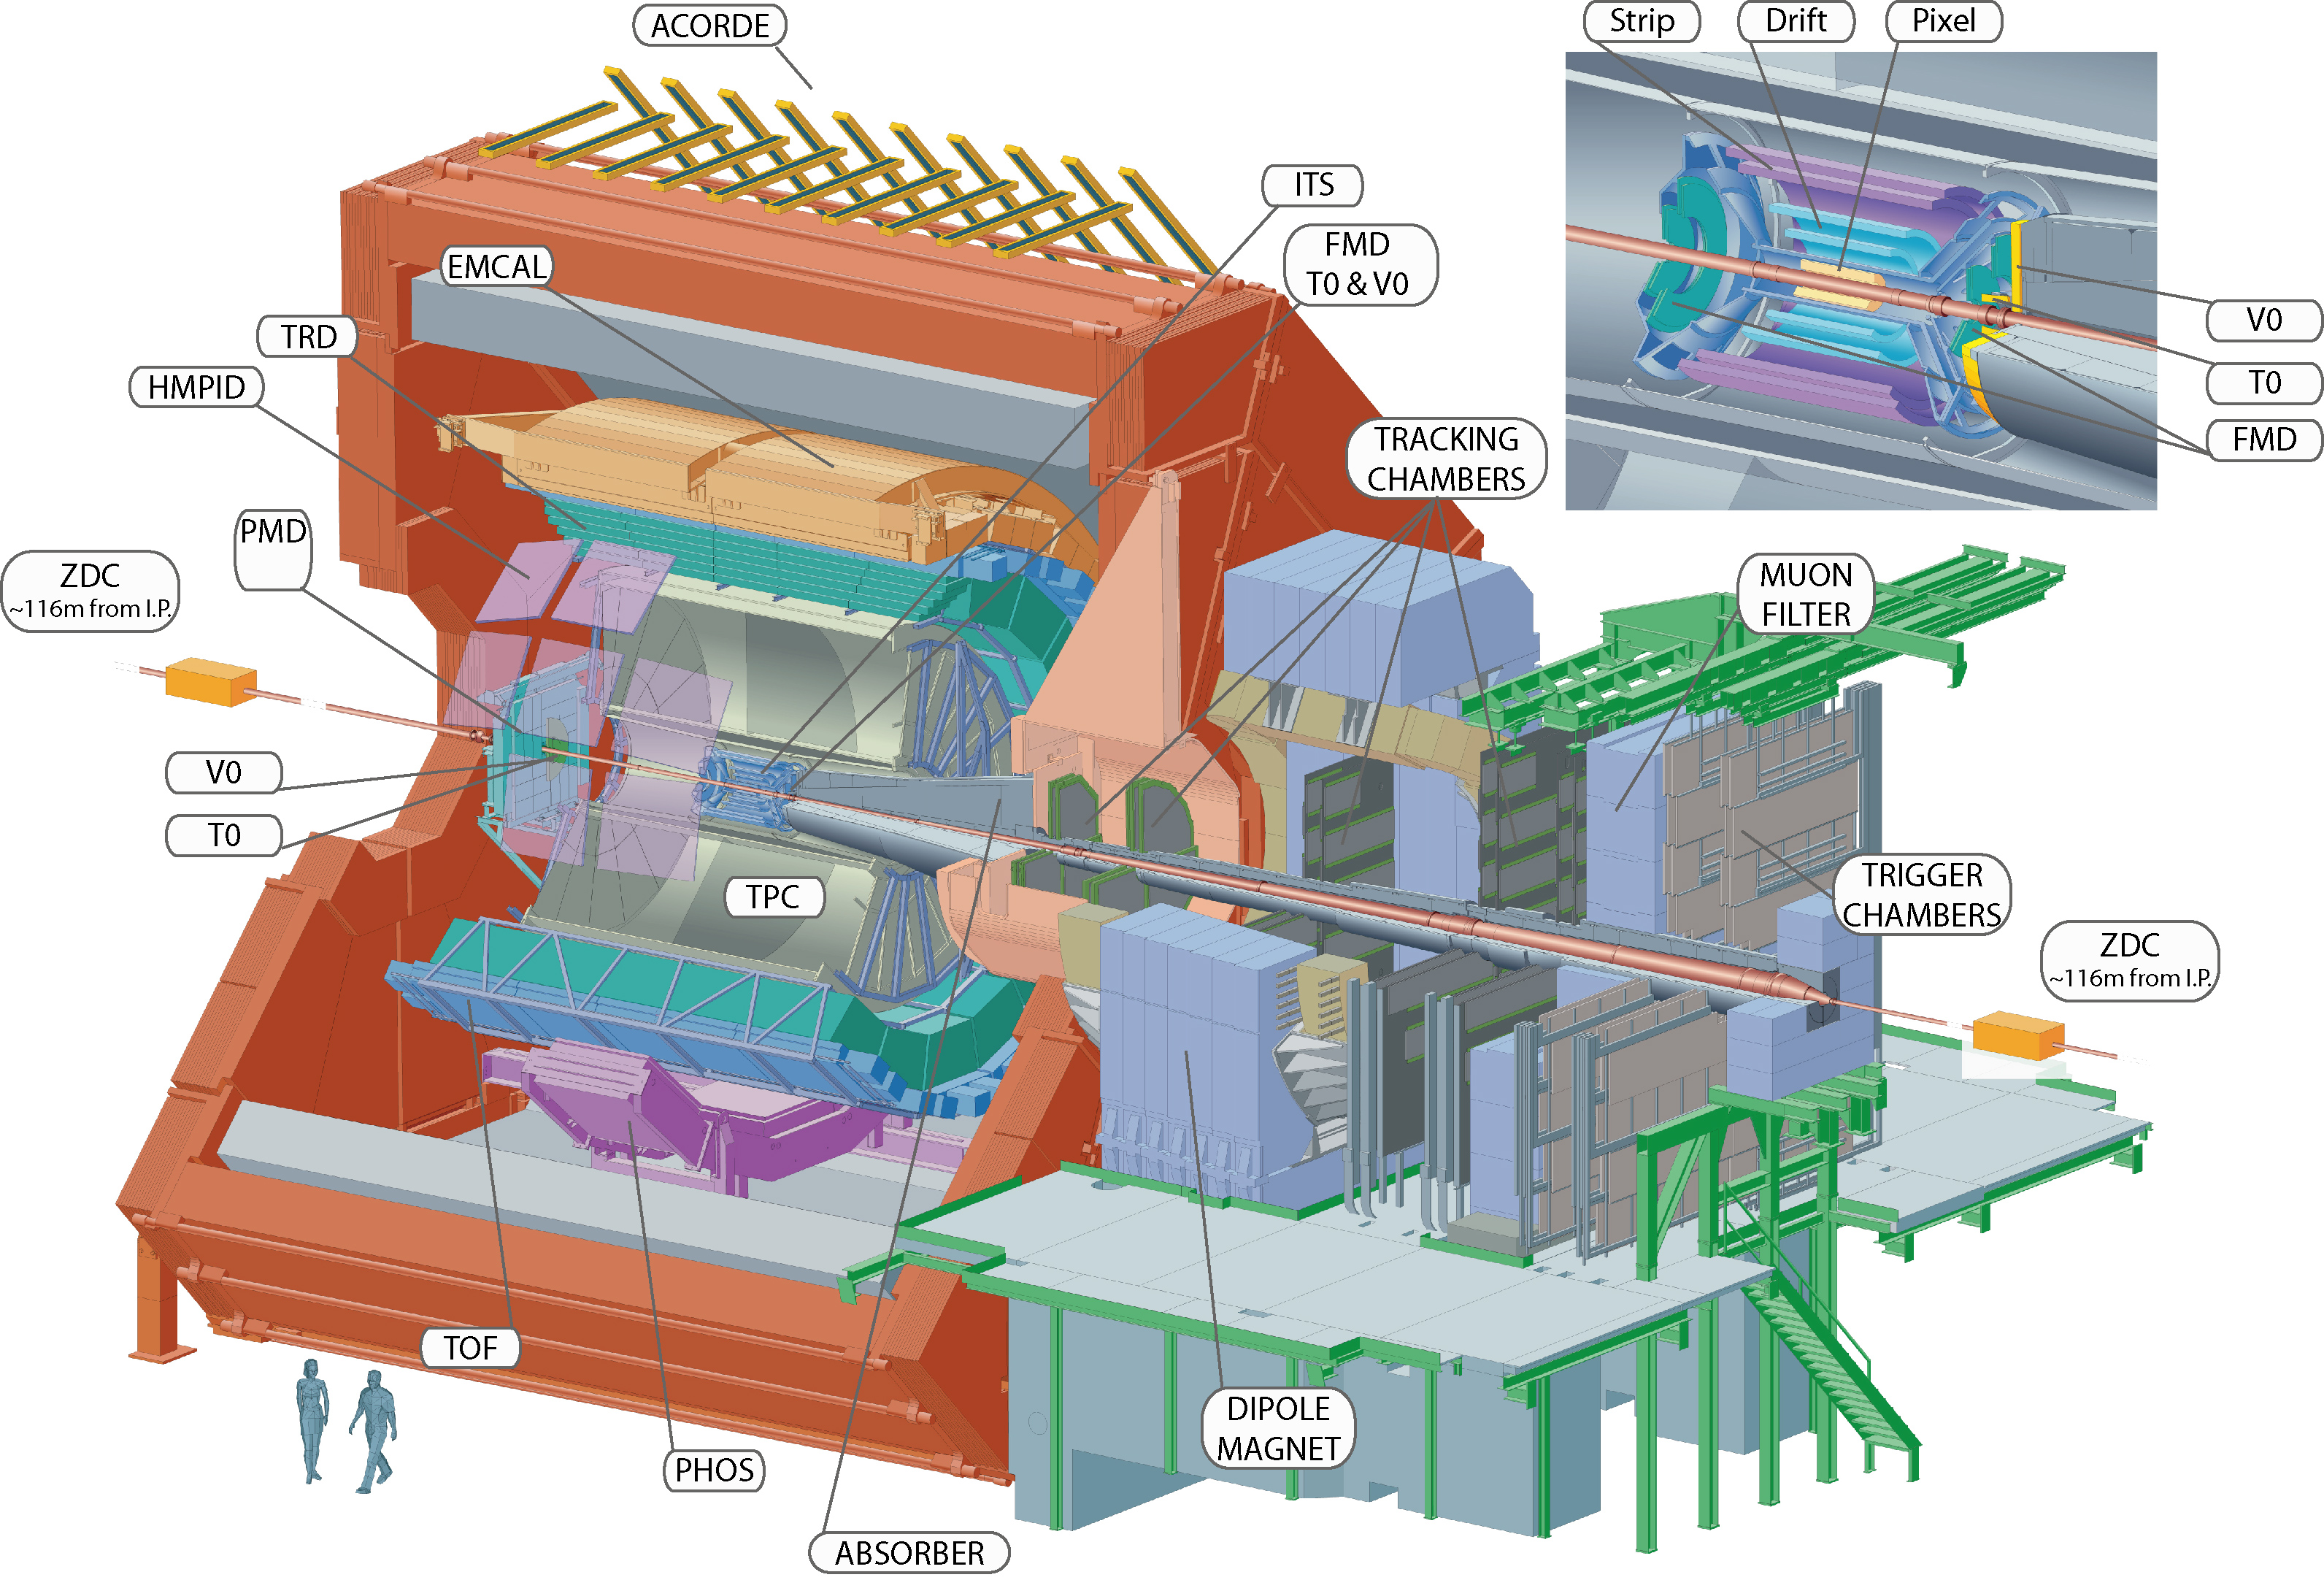
\includegraphics[width=.9\linewidth]{ALICE.jpg}
\caption{Schematische Darstellung eines Clusters. Die Ellipsenhalbachsen M20 und M02 definieren eine Ellipse, welche alle orange markierten Zellen, die zu einem Cluster geh\"ohren, umfasst.
[$https://en.wikipedia.org/wiki/ALICE_experiment]$}
\label{fig:ALICE}
\end{figure}